\graphicspath{{../../S09_Horaires_et_durees/Images}}

\themeM
\chapter{Horaires et durées}
\label{S09}

\programme%
   {\item Connaître les horaire et durées et les relations qui les lient.}
   {\item Mener des calculs impliquant des grandeurs mesurables, exprimer les résultats dans des les unités adaptées.
    \item Exprimer et vérifier la cohérence des résultats du point de vue des unités.}

\vfill

\begin{debat}{Débat : Instruments anciens de mesure de temps et de durée}
   De tous temps on a voulu mesurer le {\bf temps} et la {\bf durée}, ci-dessous figurent quelques instruments utilisés dans des époques plus ou moins lointaines.
   \tcblower
      \begin{tabular}{*{3}{C{5}}}
         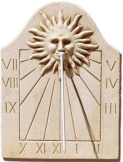
\includegraphics[height=3cm]{cadran}
         &
         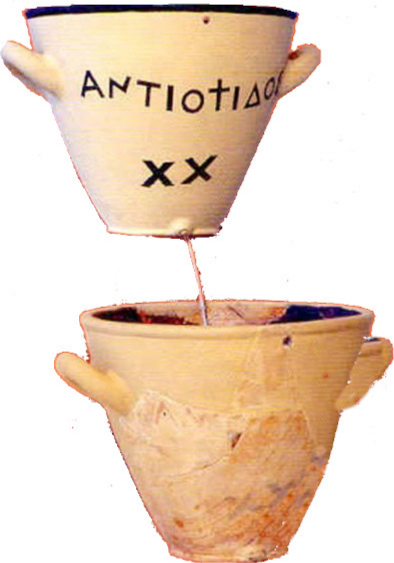
\includegraphics[height=3cm]{clepshydre.png}
         &
         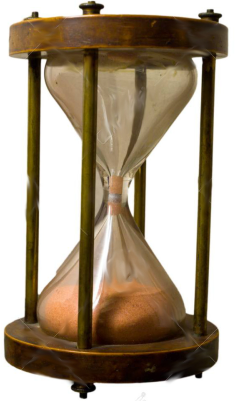
\includegraphics[height=3cm]{sablier.png} \\
         Cadran solaire & Clepsydre & Sablier \\
         1\,500 av. J.-C. & 1\,600 av. J.-C. & IX\up{e} siècle \\
         Heures du jour & Durées longues (heures) & Durées courtes (minutes) \\
      \end{tabular}
\end{debat}

\hfill {\gray Vidéo : \href{https://www.youtube.com/watch?v=8vMTE9U9z0U}{\bf Remettons les pendules à l'heure}, chaîne YouTube {\it C'est pas sorcier}.}


%%% Approche %%%
\begin{Maquette}[Cours]{Theme={Activité d'approche},Couleur={SteelBlue}}

   \AAtitre{Le temps qui passe}

      {\it Objectifs : donner un ordre de grandeur dans le domaine des durées.}

      \begin{AActivite}

         \AApartie{Les règles du jeu}
            {\singlespacing
            Pour chacune des douze situations numérotées A à L ci-dessous :
            \begin{itemize}
               \item trouver un ordre de grandeur de la durée (seconde, minute, heure, jour, mois, année ou siècle) ;
               \item identifier la couleur correspondante dans le tableau suivant :
                  \begin{center}
                        \begin{tabular}{|>{\columncolor{lightgray}}c|*{7}{C{1.5}|}}
                           \hline
                           Durée & seconde & minute & heure & jour & mois & année & siècle \\
                           \hline
                           Couleur & blanc & beige & noir & jaune & marron & rouge & bleu \\
                           & & \cellcolor{Bisque}{} & \cellcolor{Black}{} & \cellcolor{yellow}{} & \cellcolor{SaddleBrown}{} & \cellcolor{red}{} & \cellcolor{Blue}{} \\
                           \hline
                        \end{tabular}
                  \end{center}
               \item colorier les cases avec le numéro de la situation de la couleur identifiée.
            \end{itemize}}

         \AApartie{À vous de jouer !}
            \begin{multicols}{2}
               {\singlespacing
               \begin{enumerate}[label=\Alph*.]
                  \item Temps mis par la lumière du soleil pour aller jusqu'à la Terre.
                  \item Durée de chacune des quatre saisons.
                  \item Record du monde du \Lg[m]{100}.
                  \item Temps de cuisson d'un \oe uf à la coque.
                  \item Intervalle entre deux battements de c\oe ur consécutifs.
                  \item Durée d'un cycle complet de lune.
                  \item Durée d'un weekend.
                  \item Durée d'un film.
                  \item Temps mis par la Terre pour faire le tour de son étoile : le Soleil.
                  \item Âge maximum atteint par un humain.
                  \item Durée d'une grossesse.
                  \item Durée d'un entraînement de sport.
               \end{enumerate}}
            \end{multicols}
            \begin{center}
               \PixelArt[Unite=4mm,Lettres=ABCDEFGHIJKL,Largeur=18,Hauteur=29,ListeCouleurs={Bisque,Brown,White,Bisque,White,Maroon,Yellow,Black,Red,Blue,Red,Black}]{../../S09_Horaires_et_durees/Images/Mario_duree.csv}
            \end{center}

      \end{AActivite}

\end{Maquette}


%%%Trace écrite %%%
\begin{Maquette}[Cours]{Theme={Trace écrite},Couleur={0.4[SteelBlue,Black]}}

   %%%1
   \section{Unités de temps}

      Selon les situations, on indique les durées en années, mois, jours, heures, minutes, ou secondes : \par
      1 siècle = 100 ans ; 1 an = 12 mois = 365/366 jours ; 1 jour = 24 heures ; 1 heure = 60 minutes = \num{3600} secondes\dots \par
      Pour mesurer le temps ou une durée, on peut utiliser un cadran solaire, un sablier, une montre, un chronomètre\dots

   %%%2
   \section{Conversion de durées}

      La seconde (s) est l'unité du système SI permettant de caractériser une durée. Contrairement aux autres unités, elle ne suit pas un système décimal, mais hexadécimal (de base 60).

      \begin{methode*}{Convertir des durées}
         Pour convertir des heures en minutes ou des minutes en secondes ou inversement, on peut utiliser le schéma suivant : \par
         \begin{pspicture}(-3,-0.5)(11.5,3.5)
            \rnode{A}{\psframebox{durée en heures}}
            \hspace{12mm}
            \rnode{B}{\psframebox{durée en minutes}}
            \hspace{12mm}
            \rnode{C}{\psframebox{durée en secondes}}
            \nccurve[angle=90,linecolor=DodgerBlue,offset=-1mm]{A}{B}
            \naput*{\textcolor{DodgerBlue}{$\stackrel{\times60}{\longrightarrow}$}}
            \nbput*{\textcolor{DodgerBlue}{$\stackrel{\div60}{\longleftarrow}$}}
            \nccurve[angle=90,linecolor=DodgerBlue,offset=-1mm]{->}{B}{C}
            \naput*{\textcolor{DodgerBlue}{$\stackrel{\times60}{\longrightarrow}$}}
            \nbput*{\textcolor{DodgerBlue}{$\stackrel{\div60}{\longleftarrow}$}}
            \nccurve[angle=90,linecolor=Crimson]{->}{A}{C}
            \naput*{\textcolor{Crimson}{$\stackrel{\times3\,600}{\longrightarrow}$}}
            \nbput*{\textcolor{Crimson}{$\stackrel{\div3\,600}{\longleftarrow}$}}
         \end{pspicture}
         \begin{exmethode}
            \begin{itemize}
               \item Convertir 170 minutes en heures et minutes.
               \item Convertir \Temps{;;;1;25;36} en secondes.
            \end{itemize} 
            \tcblower
               \begin{itemize}
                  \item $170=2\times60+50$, donc $\Temps{;;;;170} =\Temps{;;;2;50}$.
                  \item $\Temps{;;;1;25;36} =\Temps{;;;;;3600}+25\times\Temps{;;;;;60}+\Temps{;;;;;36}$ \par
                     $\Temps{;;;1;25;36} =\Temps{;;;;;5136}$.
               \end{itemize}
         \end{exmethode}
      \end{methode*}

      Pour effectuer des additions ou soustractions de durées, on peut effectuer une opération en colonne (un peu périlleuse) ou procéder de proche en proche.
      
      \begin{exemple*}{}
         \begin{itemize}
            \item Un train part de Montpellier à \Temps{;;;8;48}. La durée du trajet pour se rendre à Paris est de \Temps{;;;3;20}. \par
               À quelle heure arrivera-t-il à Paris ? \par
               \qquad
               \begin{tabular}{ccccc}
                  & 8 & h & 4 & 8 \\
                  $+$ & 3 & h & 2 & 0 \\
                  \hline
                  1 & $\cancel{1}$ & h & $\cancel{6}$ & 8 \\
                  \multicolumn{5}{c}{\psline{->}(0.5,0.3)(-0.5,-0.1)} \\
                  1 & 2 & h & 0 & 8
               \end{tabular}
               \qquad
               \begin{tabular}{p{8cm}}
                  \small
                  On aligne les heures sous les heures, les minutes sous les minutes puis on additionne terme à terme. \\ [8mm]
                  Si le nombre de minutes est supérieur à 60, on soustrait 60 minutes et on ajoute 1 heure. \\
               \end{tabular} 
            \item Un automobiliste part de Perpignan à \Temps{;;;8;35} et arrive à Montpellier à \Temps{;;;10;20}. \par
               Quelle est la durée de son trajet ? \par \smallskip
               \qquad \Temps{;;;8;35} $\xrightarrow{+\Temps{;;;;25}}$ \Temps{;;;9;00} $\xrightarrow{+\Temps{;;;1}}$ \Temps{;;;10;00} $\xrightarrow{+\Temps{;;;;20}}$ \Temps{;;;10;20}. \par  
               La durée totale du trajet est de \Temps{;;;1;45}
         \end{itemize} 
      \end{exemple*}

      Remarque : attention à l'aspect hexadécimal de cette grandeur.
         \begin{itemize}
            \item Lorsqu'on lit \Temps{;;;1,5}, cela correspond à \Temps{;;;1} et \Temps{;;;0,5}, c'est-à-dire \Temps{;;;1;30} ($0,5\times\Temps{;;;;60} =\Temps{;;;;30}$).
            \item Inversement, \Temps{;;;2;15} ne correspond pas à \Temps{;;;2,15} mais à \Temps{;;;2,25} ($\Temps{;;;;15} =\dfrac{15}{60}\text{h} =\Temps{;;;0,25}$).
         \end{itemize}

\end{Maquette}


%%% Exercices %%%
\begin{Maquette}[Fiche,CorrigeFin,Colonnes=2]{}

   \begin{multicols}{2}

      \begin{exercice} %1
         Malak part à \Temps{;;;7;38} pour prendre le bus direction le collège Simone Veil. \par
         Elle met 6 minutes pour aller jusqu'à l'arrêt de bus, puis le trajet en bus dure 16 minutes et enfin il lui reste 4 minutes à pied. \par
         À quelle heure arrivera-t-elle au collège ?
      \end{exercice}
      
      \begin{Solution}
         Le temps de déplacement de Malak est de \par
         $\Temps{;;;;6}+\Temps{;;;;16}+\Temps{;;;;4} =\Temps{;;;;26}$. \par
         Or, $\Temps{;;;7;38}+\Temps{;;;;26} =\Temps{;;;7;64} =\Temps{;;;8;4}$. \par
         \cor{Malak devrait arriver au collège à \Temps{;;;8;4}\,\Temps{;;;;04}}.
      \end{Solution}

      
      \begin{exercice} %2
         Hugoline part du collège à pied à \Temps{;;;17;4}. \par
         Elle prévoit \Temps{;;;;15;30} pour le trajet, \Temps{;;;;5} pour acheter un pain au chocolat et \Temps{;;;;7} pour dire au revoir aux copines (et copains !). \par
         À quelle heure arrivera-t-elle chez elle ?
      \end{exercice}
      
      \begin{Solution}
         Le temps de déplacement de Hugoline est de \par
         $\Temps{;;;;15;30}+\Temps{;;;;5}+\Temps{;;;;7} =\Temps{;;;;27;30}$. \par
         Or, $\Temps{;;;17;4}+\Temps{;;;;27;30} =\Temps{;;;17;31;30}$. \par
         \cor{Hugoline devrait arriver chez elle à \Temps{;;;17;31;30}}.
      \end{Solution}
      
      
      \begin{exercice} %3
         Safae part en promenade à \Temps{;;;9;20}. \par
         Elle rentre à \Temps{;;;12;15}, ne s'étant arrêtée pour se reposer que lors de trois pauses de \Temps{;;;;5} chacune. \par
         Pendant combien de temps a-t-elle marché ?
      \end{exercice}
      
      \begin{Solution}
         $\Temps{;;;9;20} \quad \xrightarrow{+\Temps{;;;;40}} \quad \Temps{;;;10;0}$ \par
         $\Temps{;;;10;0} \quad \xrightarrow{+\Temps{;;;2;15}} \quad \Temps{;;;12;15}$ \par
         La promenade de Safae a duré \Temps{;;;2;55}. \par
         Or, il s'est arrêtée $3\times\Temps{;;;;5} =\Temps{;;;;15}$ \par
         donc, \cor{elle a marché durant \Temps{;;;2;40}\,\Temps{;;;;40}}.
      \end{Solution}
      
      
      \begin{exercice} %4
         Convertir les durées données ci-dessous en minutes.
         \begin{enumerate}
            \item \Temps{;;;1;56}.
            \item \Temps{;;2;;25}.
            \item \Temps{;;1;20;3}.
         \end{enumerate}
      \end{exercice}
      
      \begin{Solution}
         \begin{enumerate}
            \item $\Temps{;;;1;56}. =1\times\Temps{;;;;60}+\Temps{;;;;56} =\cor{\Temps{;;;;116}}$.
            \item $\Temps{;;2;;25} =2\times24\times\Temps{;;;;60}+\Temps{;;;;25}$ \par
               \quad $=\Temps{;;;;2880}+\Temps{;;;;25} =\cor{\Temps{;;;;2905}}$.
            \item $\Temps{;;1;20;3} =24\times\Temps{;;;;60}+20\times\Temps{;;;;60}+\Temps{;;;;3}$ \par
               \quad $=\Temps{;;;;1440}+\Temps{;;;;1200}+\Temps{;;;;3} =\cor{\Temps{;;;;2643}}$.
         \end{enumerate}
      \end{Solution}
      
      
      \begin{exercice} %5
         Convertir les durées données ci-dessous en heures et minutes.
         \begin{enumerate}
            \item \Temps{;;;;156}.
            \item \Temps{;;;;296}.
            \item \Temps{;;;;1603}.
         \end{enumerate}
      \end{exercice}
      
      \begin{Solution}
         \begin{enumerate}
            \item $\Temps{;;;;156} =2\times\Temps{;;;;60}+\Temps{;;;;36} =\cor{\Temps{;;;2;36}}$.
            \item $\Temps{;;;;296} =4\times\Temps{;;;;60}+\Temps{;;;;56} =\cor{\Temps{;;;4;46}}$.
            \item $\Temps{;;;;1603} =26\times\Temps{;;;;60}+\Temps{;;;;43}$ \par
               \quad $=\Temps{;;;26;43} =\cor{\Temps{;;1;2;43}}$.
         \end{enumerate}
      \end{Solution}
      
      
      \begin{exercice} %6
         Convertir les durées données ci-dessous en heures et minutes.
         \begin{enumerate}
            \item \Temps{;;;1,5}.
            \item \Temps{;;;2,25}.
            \item \Temps{;;;0,3}.
         \end{enumerate}
      \end{exercice}
      
      \begin{Solution}
         \begin{enumerate}
            \item $\Temps{;;;1,5} =\cor{\Temps{;;;1;30}}$.
            \item $\Temps{;;;2,25} =\cor{\Temps{;;;2;15}}$.
            \item $\Temps{;;;0,3} =0,3\times\Temps{;;;;60} =\cor{\Temps{;;;;18}}$.
         \end{enumerate}
      \end{Solution}
      
      
      \begin{exercice}[Dur] %4
         Convertir les durées données ci-dessous en heures décimales.
         \begin{enumerate}
            \item $\Temps{;;;6;30}$.
            \item $\Temps{;;;2;45}$.
            \item $\Temps{;;;8;33}$.
         \end{enumerate}
      \end{exercice}
      
      \begin{Solution}
         \begin{enumerate}
            \item $\Temps{;;;6;30} =\cor{\Temps{;;;6,5}}$.
            \item $\Temps{;;;2;45} =\cor{\Temps{;;;2,75}}$. \smallskip
            \item $\Temps{;;;8;33} =\Temps{;;;8}+\frac{33}{60}\text{h} =\cor{\Temps{;;;8,55}}$.
         \end{enumerate}
      \end{Solution}
       
      
      \begin{exercice} %8
         Effectuer les calculs suivants :
         \begin{enumerate}
            \item $\Temps{;;;3}\,\Temps{;;;;45}+\Temps{;;;5}\,\Temps{;;;;13}$
            \item $\Temps{;;;5}\,\Temps{;;;;38}+\Temps{;;;9}\,\Temps{;;;;43}$
            \item $\Temps{;;;11}\,\Temps{;;;;28}-\Temps{;;;7}\,\Temps{;;;;22}$
            \item $\Temps{;;;15}\,\Temps{;;;;35}-\Temps{;;;9}\,\Temps{;;;;49}$
         \end{enumerate}
      \end{exercice}
      
      \begin{Solution}
         \begin{enumerate}
            \item $\Temps{;;;3}+\Temps{;;;5} =\Temps{;;;8}$ et $\Temps{;;;;45}+\Temps{;;;;13} =\Temps{;;;;58}$ \par
               donc, $\Temps{;;;3}\,\Temps{;;;;45}+\Temps{;;;5}\,\Temps{;;;;13} =\cor{\Temps{;;;8;58}}$.
            \item $\Temps{;;;5}+\Temps{;;;9} =\Temps{;;;14}$ et \par
               $\Temps{;;;;38}+\Temps{;;;;43} =\Temps{;;;;81} =\Temps{;;;1;21}$ \par
               donc, $\Temps{;;;5;38}+\Temps{;;;9;43} =\cor{\Temps{;;;15;21}}$.
            \item $\Temps{;;;7;22} \quad \xrightarrow{+\Temps{;;;;38}} \quad \Temps{;;;8;0}$ \par
               \quad\, $\Temps{;;;8;0} \quad \xrightarrow{+\Temps{;;;3;28}} \quad \Temps{;;;11;28}$ \par
               $\Temps{;;;11;28}-\Temps{;;;7;22} =\Temps{;;;3;66} =\cor{\Temps{;;;4;6}}$.
            \item $\Temps{;;;9;39} \quad \xrightarrow{+\Temps{;;;;11}} \quad \Temps{;;;10;0}$ \par
               \quad\, $\Temps{;;;10;0} \quad \xrightarrow{+\Temps{;;;5;35}} \quad \Temps{;;;15;35}$ \par  
               $\Temps{;;;15;35}-\Temps{;;;9;49} =\cor{\Temps{;;;5;46}}$.
         \end{enumerate}
      \end{Solution}


      \begin{exercice} %9
         Dans une usine, une machine met \Temps{;;;;5;26} pour fabriquer une pièce.
         \begin{enumerate}
            \item Combien de temps met-elle pour fabriquer 5 pièces ?
            \item Combien de temps met-elle pour en fabriquer 10 ?
            \item Combien de temps met-elle pour en fabriquer 20 ?
            \item Combien de temps met-elle pour en fabriquer 100 ?
            \item Combien la machine aura-t-elle fabriqué de pièces si elle fonctionne \Temps{;;;8} sans s’arrêter ?
            \item Une nouvelle machine, qui vient d’arriver, met deux fois moins de temps pour fabriquer la même pièce. Quel temps met-elle pour fabriquer la pièce ?
         \end{enumerate}
      \end{exercice}
      
      \begin{Solution}
         \begin{enumerate}
            \item $5\times\Temps{;;;;5} =\Temps{;;;;25}$ et $5\times\Temps{;;;;;26} =\Temps{;;;;;130} =\Temps{;;;;2;10}$. \par
               $\Temps{;;;;25}+\Temps{;;;;2;10} =\cor{\Temps{;;;;27;10}}$.
            \item $2\times(\Temps{;;;;27;10}) =\cor{\Temps{;;;;54;20}}$.
            \item $2\times(\Temps{;;;;54;20}) =\Temps{;;;;108;40} =\cor{\Temps{;;;1;48;40}}$.
            \item $10\times(\Temps{;;;;54;20}) =\Temps{;;;;540;200} =\cor{\Temps{;;;9;3;20}}$.
            \item $\Temps{;;;8} =8\times\Temps{;;;;;3600} =\Temps{;;;;;28800}$ \par
               et $\Temps{;;;;5;26} =5\times\Temps{;;;;;60}+\Temps{;;;;;26} =\Temps{;;;;;326}$. \par
               Or, $\num{28800}\div326 \approx88,34$ donc, \cor{la machine aura fabriqué 88 pièces en \Temps{;;;8}}.
            \item La moitié de \Temps{;;;;5} vaut \Temps{;;;;2;30} et la moitié de \Temps{;;;;;26} vaut \Temps{;;;;;13} donc, \cor{la machine met \Temps{;;;;2;43}}.
         \end{enumerate}
      \end{Solution}
      
      
      \begin{exercice}[Dur] %10
         Résolution de problème : des robinets qui coulent. \par
         On dispose de deux robinets.
         \begin{itemize}
            \item Le premier est capable de remplir un réservoir d’eau de \Capa{24} en 1 minute.
            \item Le second peut remplir ce même réservoir en 2 minutes.
         \end{itemize}
         En ouvrant les deux robinets au même moment, combien de temps faudrait-il pour remplir un jacuzzi avec \Capa{1080} d’eau ? \par
         \begin{minipage}{4cm}
            \begin{enumerate}
               \item[a.] 15 min.
               \item[b.] 67,5 min.
               \item[c.] 135 min.
               \item[d.] 30 min.
            \end{enumerate}
         \end{minipage}
         \begin{minipage}{2cm}
            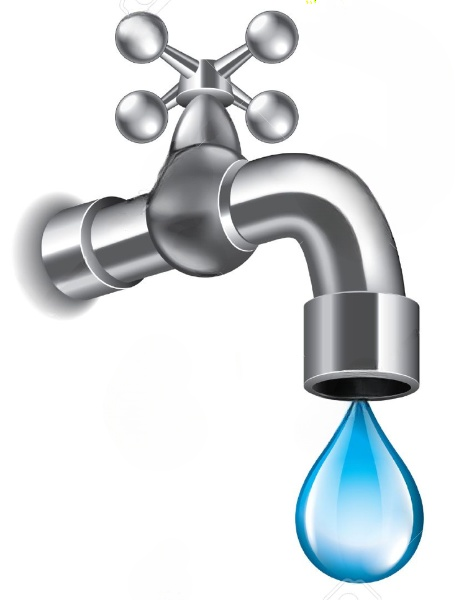
\includegraphics[width=2cm]{robinet}
         \end{minipage}
      \end{exercice}
      
      \begin{Solution}
         Pour un volume à remplir, le robinet R1 met deux fois moins de temps que le robinet R2. Donc, pendant le temps total, R1 remplit deux \og unités de volume \fg{} pendant que R2 n'en remplit qu’une : \par \smallskip
         \ModeleBarre[Largeur=2.5cm]{PowderBlue 3 {"\Capa{1080}"}}{DeepSkyBlue 1 "R1" DeepSkyBlue 1 "R1" LightSkyBlue 1 "R2"} \par
         En partageant le volume total en trois parties égales, on trouve $\Capa{1080}\div3 =\Capa{360}$. \par
         R2 remplit un tiers du volume total du jacuzzi : \Capa{360}. \par
         Or, $360\div12 =30$. Sachant que R2 remplit \Capa{12} en \Temps{;;;;1}, il remplit \Capa{360} en \Temps{;;;;30}. \par
         \cor{La réponse est 30 minutes (d)}.
      \end{Solution}

   \end{multicols}

\end{Maquette}


%%% Récré %%%
\begin{Maquette}[Cours]{Theme={Activité récréative},Couleur={IndianRed}}
    
   \ARtitre{L'horloge de Mengenlehreuhr}

      \ARpartie{Présentation}  
         La {\bf Mengenlehreuhr} (en allemand \og Horloge de la théorie du jeu \fg) ou {\bf Berlin-Uhr} (\og Horloge de Berlin \fg) est la première horloge publique au monde qui indique l'heure au moyen de champs lumineux colorés, ce qui lui a valu d'entrer dans le livre Guinness des records lors de son installation le 17 juin 1975. \par
         \hfill{\it \small Source : \href{https://en.wikipedia.org/wiki/Mengenlehreuhr}{wikipedia}}

      \ARpartie{recherche}
         À partir des images suivantes représentant l'horloge à différents moments de la journée, déterminer le fonctionnement de l'horloge. Par groupe, vous construirez une affiche récapitulant vos recherches.
         \vfill
         \begin{center}
            {\psset{unit=0.54}
            \begin{minipage}{6cm}  
               \begin{pspicture}(0,-1.5)(11,13.8)
                  \rput(5.5,6.5){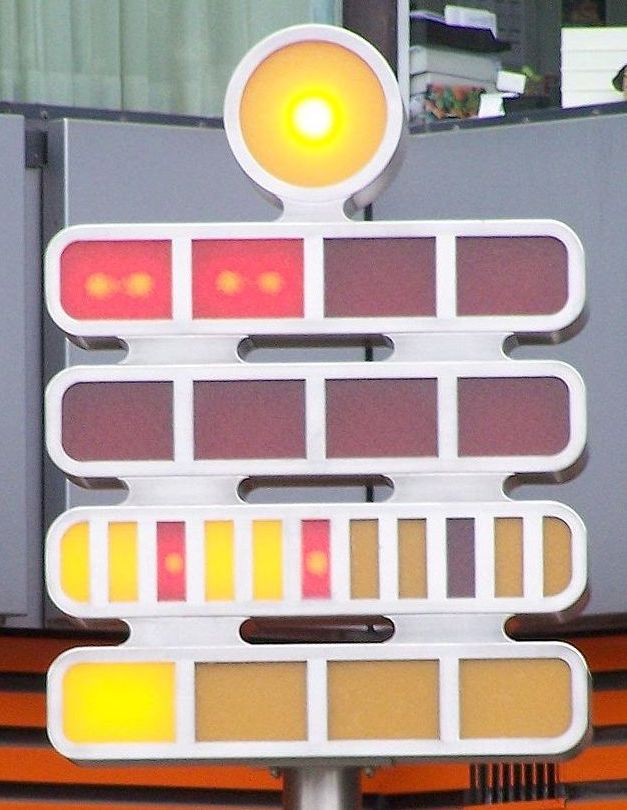
\includegraphics[width=6.7cm]{horloge_Berlin}}
               \end{pspicture}
            \end{minipage}
            \hspace{3cm}
            \begin{minipage}{6cm}  
               \begin{pspicture}(0,-1)(11,13.8)
                  \psset{linecolor=yellow,fillstyle=solid,framearc=0.35}
                     \psframe*(0,0)(2.75,2) %m1
                     \psframe*(0,2.8)(5,4.8) %m5
                     \pscircle*(5.5,12.54){1.6}
                  \psset{linecolor=OrangeRed}
                     \psframe*(2,2.8)(3,4.8) \psframe*(5,2.8)(6,4.8) %mi
                     \psframe*(0,8.4)(5.5,10.4) %h5  
                  \horloge
                  \rput(5.5,-1){\large Il est 10h31}
               \end{pspicture}
            \end{minipage}
            \vfill
            \begin{minipage}{6cm}  
               \begin{pspicture}(0,-1)(11,15.5)
                  \psset{linecolor=yellow,fillstyle=solid,framearc=0.35}
                     \psframe*(0,0)(2.75,2) %m1
                     \psframe*(0,2.8)(1,4.8) %m5
                  \psset{linecolor=OrangeRed}
                     \psframe*(0,5.6)(2.75,7.6) %h1
                     \psframe*(0,8.4)(2.75,10.4) %h5  
                  \horloge
                  \rput(5.5,-1){\large Il est 6h06}
               \end{pspicture}
            \end{minipage}
            \hspace{3cm}
            \begin{minipage}{6cm}  
               \begin{pspicture}(0,-1)(11,15)
                  \psset{linecolor=yellow,fillstyle=solid,framearc=0.35}
                     \psframe*(0,2.8)(11,4.8) %m5
                  \psset{linecolor=OrangeRed}
                     \psframe*(2,2.8)(3,4.8) \psframe*(5,2.8)(6,4.8) \psframe*(8,2.8)(9,4.8) %mi
                     \psframe*(0,5.6)(8.25,7.6) %h1
                  \horloge
                  \rput(5.5,-1){\large Il est 3h55}
               \end{pspicture}
            \end{minipage}
            \vfill}
         \end{center}

\end{Maquette}